\documentclass[areasetadvanced]{scrartcl}

\usepackage[utf8]{inputenc}
\usepackage[T2A]{fontenc}
\usepackage[english,russian]{babel}
\usepackage{xcolor}

\usepackage[footskip=1cm,left=25mm, right=15mm, top=20mm, bottom=20mm]{geometry}
\usepackage{setspace}
\usepackage{amsmath, amssymb} 
\usepackage{graphicx}
\usepackage{tikz}
\usetikzlibrary{arrows.meta}
\usepackage{float}
\usepackage{dashrule}
\usepackage{fancyhdr} 
\usepackage{hyperref} 
\usepackage{parskip}
\usepackage{textcomp, enumitem}
\usepackage{indentfirst}
\usepackage{graphicx}
\usepackage{algorithm}
\usepackage{algpseudocode}
\usepackage{array} 
\usepackage{geometry}
\usepackage{afterpage}
\usepackage{minted}
\setcounter{secnumdepth}{3} 
\setcounter{tocdepth}{3}    
\usepackage{listings} 
\usepackage{booktabs}
\usepackage{paracol} % параллельные колонки (левая/правая)

\newcommand{\icon}[1]{\includegraphics[height=1.2em]{#1}}

\tikzstyle{block} = [rectangle, rounded corners, minimum width=3cm, minimum height=1cm, text centered, draw=black, fill=lightgray]

\setkomafont{sectioning}{\normalfont\bfseries} 
\setkomafont{section}{\normalfont\Large\bfseries}
\setkomafont{subsection}{\normalfont\large\bfseries}
\setkomafont{subsubsection}{\normalfont\large\bfseries}
\setkomafont{paragraph}{\normalfont\large\bfseries} 
\newcommand{\twosideheading}[2]{%
  \noindent
  \begin{minipage}[t]{0.5\textwidth}\raggedright\small #1\end{minipage}%
  \begin{minipage}[t]{0.5\textwidth}\raggedleft\Large\bfseries #2\end{minipage}\\[-0.2em]
  \hrule
  \vspace{0.8em}
}
\lstset{
  language=Haskell,
  basicstyle=\ttfamily\small,
  keywordstyle=\color{blue}\bfseries,
  stringstyle=\color{red},
  commentstyle=\color{green!70!black},
  numbers=left,
  numberstyle=\tiny,
  stepnumber=1,
  numbersep=10pt,
  showstringspaces=false,
  breaklines=true,
  frame=single
}

\lstdefinelanguage{Lua}{
    keywords={function, end, if, then, else, elseif, for, while, do, repeat, until, break, return, local, and, or, not, true, false, nil},
    keywordstyle=\color{blue}\bfseries,
    stringstyle=\color{red},
    commentstyle=\color{green!70!black},
    morestring=[s]{"}{"},
    morestring=[s]{'}{'},
    morecomment=[l]{--},
    morecomment=[s]{--[[}{]]},
    basicstyle=\ttfamily\small,
    numbers=left,
    numberstyle=\tiny,
    stepnumber=1,
    numbersep=10pt,
    showstringspaces=false,
    breaklines=true,
    frame=single
}

\lstdefinestyle{py}{
    language=Python,
    basicstyle=\ttfamily\small,
    keywordstyle=\color{blue}\bfseries,
    stringstyle=\color{red},
    commentstyle=\color{green!70!black},
    numbers=left,
    numberstyle=\tiny,
    stepnumber=1,
    numbersep=10pt,
    showstringspaces=false,
    breaklines=true,
    frame=single
}

\setlength{\parindent}{1.25cm}
\setcounter{tocdepth}{3}
\begin{document}
\sloppy
	\thispagestyle{empty}
	\begin{center}
		\large{МИНОБРНАУКИ РОССИИ} \par
		\vspace{0.3cm}
		\normalsize
		{ФЕДЕРАЛЬНОЕ ГОСУДАРСТВЕННОЕ АВТОНОМНОЕ ОБРАЗОВАТЕЛЬНОЕ УЧРЕЖДЕНИЕ ВЫСШЕГО ОБРАЗОВАНИЯ} \par
		\vspace{0.3cm}
		\textbf{\guillemotleft САНКТ-ПЕТЕРБУРГСКИЙ ПОЛИТЕХНИЧЕСКИЙ}
		\textbf{УНИВЕРСИТЕТ ПЕТРА ВЕЛИКОГО\guillemotright} \par
		\vspace{0.3cm}
		{Институт компьютерных наук и кибербезопасности}\par
		{Высшая школа технологий искусственного интеллекта}\par
	\end{center}
	\vfill
	\begin{center}
		{\large Отчёт по дисциплине \guillemotleft Генетические алгоритмы\guillemotright}\par
		\vspace{1cm}
		\Huge Лабораторная работа №6\par
		\vspace{0.5cm}
		{\huge \guillemotleft Оптимизация путей на графах с помощью муравьиных алгоритмов\guillemotright \\
        Вариант №17}\par
	\end{center}
	\vfill
	\begin{flushleft}
		Студент: \hspace{1.8cm} \rule[0pt]{2.5cm}{0.5pt}\hfill Салимли Айзек Мухтар Оглы\par
		\vspace{1.5cm}
		Преподаватель: \hspace{0.55cm} \rule[0pt]{2.5cm}{0.5pt}\hfill  Большаков Александр Афанасьевич
	\end{flushleft}
	\vspace{0.5cm}
	\begin{flushright}
		\guillemotleft \rule[0pt]{0.8cm}{0.5pt}\guillemotright \rule[0pt]{2cm}{0.5pt} 20\rule[0pt]{0.5cm}{0.5pt} г.
	\end{flushright}
	\vfill
	\begin{center}
		Санкт-Петербург, 2025
	\end{center}
	\newpage
	\tableofcontents
	\newpage

\section*{Введение}
\addcontentsline{toc}{section}{Введение}
Муравьиные алгоритмы представляют собой класс метаэвристических методов
оптимизации, основанных на моделировании поведения колоний муравьев в природе. Эти алгоритмы были разработаны для решения сложных комбинаторных задач
оптимизации, в частности задач поиска путей на графах.

Основная идея муравьиных алгоритмов заключается в использовании коллективного поведения искусственных агентов (муравьев), которые взаимодействуют через отложение феромонов. Каждый муравей строит потенциальное решение задачи,
а концентрация феромона на ребрах графа отражает «качество» этих решений. Чем выше концентрация феромона на определенном ребре, тем более привлекательным оно становится для последующих муравьев.

\textbf{Цель работы}: изучить принципы работы муравьиных алгоритмов,реализовать их для решения поставленной задачи и провести анализ полученных результатов.

\newpage
\section{Постановка задачи}

\textbf{Цель лабораторной работы:}
\begin{enumerate}
    \item Реализовать с использованием муравьиного алгоритма решение задачи коммивояжера (TSP);
    \item Представить графически найденное решение и график сходимости алгоритма;
    \item Сравнить муравьиный алгоритм с генетическим алгоритмом используемом в работе №3.
\end{enumerate}

\textbf{Набор данных:}
\begin{itemize}
    \item Набор координат: 29 городов в Заподной Сахаре;
    \item Тип данных: эвклидовы координаты городов.
\end{itemize}

\textbf{Ограничение:}
\begin{itemize}
    \item Вид представления: Представление пути
\end{itemize}

\newpage
\section{Теоретические сведения}
Задача коммивояжера (ЗК) считается классической NP-трудной задачей комбинаторной оптимизации, для решения которой эффективно применяются муравьиные алгоритмы.
Оптимальное решение — такая перестановка городов, при которой длина замкнутого маршрута минимальна.

\subsection{Основные понятия муравьиных алгоритмов}
Муравьиные алгоритмы представляют собой класс вероятностных метаэвристических методов, основанных на моделировании поведения колоний муравьев в природе. Основная идея заключается в коллективном поведении простых агентов (искусственных муравьев), которые взаимодействуют через механизм феромонов для решения сложных оптимизационных задач.

\subsubsection{Биологическое обоснование}
В природе муравьи способны находить кратчайшие пути от гнезда к источникам пищи благодаря феномену, известному как «феромонная тропа». Муравьи откладывают феромоны на пройденном пути, и другие муравьи с большей вероятностью следуют по направлениям с более высокой концентрацией этого химического вещества. Со временем более короткие пути накапливают больше феромона, становясь предпочтительными.

\subsubsection{Простой муравьиный алгоритм (SACO)}
Рассмотрим простой муравьиный алгоритм для задачи поиска пути в графе.

\subsubsection{Инициализация}
На начальном этапе феромонная матрица инициализируется малыми случайными значениями:
$\tau_{ij}(0) = \text{random}(0.1,0.5)$
Муравьи размещаются в начальных вершинах графа, и начинается итерационный процесс поиска решения.

\subsubsection{Построение решений}
Каждый муравей $k$ строит решение, последовательно выбирая следующую вершину согласно вероятностному правилу:
\begin{equation}
p^k_{ij}(t) =
\begin{cases}
\frac{[\tau_{ij}(t)]^\alpha}{\sum_{l \in N^k_i} [\tau_{il}(t)]^\alpha}, & \text{если } j \in N^k_i \\
0, & \text{иначе}
\end{cases}
\end{equation}
где:
\begin{itemize}
\item $N^k_i$ — множество вершин, доступных из вершины $i$ для муравья $k$
\item $\alpha$ — параметр, определяющий влияние феромона ($\alpha \geq 0$)
\item $\tau_{ij}(t)$ — концентрация феромона на ребре $(i,j)$ в момент времени $t$
\end{itemize}

\subsubsection{Обновление феромона}
После построения всех решений выполняется обновление феромонной матрицы:
1. Испарение феромона:
\begin{equation}
\tau_{ij}(t) \leftarrow (1-\rho) \cdot \tau_{ij}(t)
\end{equation}
где $\rho \in [0,1]$ — коэффициент испарения.
2. Отложение феромона:
\begin{equation}
\tau_{ij}(t+1) = \tau_{ij}(t) + \sum_{k=1}^{m} \Delta \tau^k_{ij}(t)
\end{equation}
Количество откладываемого феромона обратно пропорционально длине пути:
\begin{equation}
\Delta \tau^k_{ij}(t) = \frac{1}{L_k(t)}
\end{equation}
где $L_k(t)$ — длина пути, построенного муравьем $k$.

\subsection{МА в задаче коммивояжера}
При решении задачи коммивояжера учитываются особенности:
\begin{itemize}
\item Маршрут должен быть замкнутым (возврат в начальный город)
\item Все города должны быть посещены ровно один раз
\item Минимизируется общая длина маршрута
\end{itemize}

\subsection{Критерии остановки алгоритма}
В практических реализациях используются следующие критерии остановки:
\begin{itemize}
\item Достижение максимального числа итераций
\item Нахождение решения с приемлемым качеством
\item Стабилизация решения (все муравьи следуют одним маршрутом)
\item Отсутствие улучшений в течение заданного числа итераций
\end{itemize}

\subsection{Влияние параметров алгоритма}
Параметр $\alpha$:
\begin{itemize}
\item Большие значения усиливают влияние феромона
\item Может приводить к преждевременной сходимости
\item Малые значения увеличивают случайность поиска
\end{itemize}
Параметр $\rho$ (испарение):
\begin{itemize}
\item Большие значения ускоряют «забывание» плохих решений
\item Малые значения сохраняют историю поиска
\item При $\rho = 1$ алгоритм вырождается в случайный поиск
\end{itemize}

\newpage
\section{Программная реализация}

\subsection{Архитектура программы}
Программа реализована на языке Python для решения задачи коммивояжера с использованием муравьиного алгоритма и состоит из следующих основных компонентов:
\begin{itemize}
\item Загрузка данных — функция \texttt{load\_cities\_coords} для обработки координат 29 городов
\item Матрица расстояний — функция \texttt{compute\_distance\_matrix} для вычисления евклидовых расстояний между городами
\item Муравьиный алгоритм — класс \texttt{AntColonyTSP} с полной реализацией алгоритма оптимизации
\item Визуализация результатов — функции \texttt{plot\_tour\_comparison} и \texttt{plot\_convergence} для графического анализа
\end{itemize}

\subsection{Структура данных}

\subsubsection{Загрузка координат}
Функция для загрузки координат 29 городов из предоставленных данных.

\begin{lstlisting}[language=Python]
def load_cities_coords():
    coords_str = """1 20833.3333 17100.0000
    2 20900.0000 17066.6667
    ...
    29 27462.5000 12992.2222"""
    
    lines = coords_str.strip().split('\n')
    coords = []
    for line in lines:
        parts = line.strip().split()
        x, y = float(parts[1]), float(parts[2])
        coords.append((x, y))
    return np.array(coords)
\end{lstlisting}

\subsubsection{Матрица расстояний}
Вычисление матрицы евклидовых расстояний между всеми парами городов.

\begin{lstlisting}[language=Python]
def compute_distance_matrix(cities):
    n = len(cities)
    dist = np.zeros((n, n))
    for i in range(n):
        for j in range(i + 1, n):
            dx = cities[i][0] - cities[j][0]
            dy = cities[i][1] - cities[j][1]
            d = math.sqrt(dx * dx + dy * dy)
            dist[i][j] = d
            dist[j][i] = d
    return dist
\end{lstlisting}

\subsection{Алгоритмическая реализация}

\subsubsection{Класс муравьиного алгоритма}
Основной класс, реализующий муравьиный алгоритм для решения TSP.

\begin{lstlisting}[language=Python]
class AntColonyTSP:
    def __init__(self, distances, n_ants=50, n_iterations=500, 
                 decay=0.3, alpha=1., beta=3., max_stagnation=30):
        self.distances = distances
        self.n_cities = len(distances)
        self.n_ants = n_ants
        self.n_iterations = n_iterations
        self.decay = decay
        self.alpha = alpha
        self.beta = beta
        self.max_stagnation = max_stagnation
        self.pheromone = np.ones((self.n_cities, self.n_cities)) * 0.1
        self.best_path = None
        self.best_length = float('inf')
        self.history = []
        self.stagnation_counter = 0
\end{lstlisting}

Параметры алгоритма:
\begin{itemize}
\item \texttt{n\_ants} — количество муравьев в колонии
\item \texttt{n\_iterations} — максимальное количество итераций
\item \texttt{decay} — коэффициент испарения феромона
\item \texttt{alpha} — влияние феромона на выбор пути
\item \texttt{beta} — влияние эвристической информации
\item \texttt{max\_stagnation} — критерий остановки при стагнации
\end{itemize}

\subsubsection{Основной цикл алгоритма}
Реализация основного цикла муравьиного алгоритма.

\begin{lstlisting}[language=Python]
def run(self):
    prev_best = float('inf')
    for it in range(self.n_iterations):
        all_paths = []
        for _ in range(self.n_ants):
            path = self._construct_solution()
            length = self._path_length(path)
            all_paths.append((path, length))
            if length < self.best_length:
                self.best_length = length
                self.best_path = path.copy()
        
        if self.best_length < prev_best:
            prev_best = self.best_length
            self.stagnation_counter = 0
        else:
            self.stagnation_counter += 1
        
        self._update_pheromone(all_paths)
        self.pheromone *= (1 - self.decay)
        self.history.append(self.best_length)
        
        if self.stagnation_counter >= self.max_stagnation:
            break
    
    return self.best_path, self.best_length, self.history
\end{lstlisting}

Ключевые особенности:
\begin{itemize}
\item Адаптивная остановка — алгоритм прекращает работу при достижении максимального числа итераций или при стагнации
\item Элитизм — сохранение лучшего решения на каждой итерации
\item Динамическое обновление — регулярное обновление феромонов и проверка улучшений
\end{itemize}

\subsubsection{Построение решения}
Метод построения маршрута для одного муравья.

\begin{lstlisting}[language=Python]
def _construct_solution(self):
    start = random.randint(0, self.n_cities - 1)
    path = [start]
    visited = {start}
    current = start
    
    for _ in range(self.n_cities - 1):
        next_city = self._select_next(current, visited)
        if next_city is None:
            break
        path.append(next_city)
        visited.add(next_city)
        current = next_city
    
    path.append(start)
    return path
\end{lstlisting}

\subsubsection{Выбор следующего города}
Вероятностный выбор следующего города на основе феромонов и эвристики.

\begin{lstlisting}[language=Python]
def _select_next(self, current, visited):
    unvisited = [j for j in range(self.n_cities) if j not in visited]
    if not unvisited:
        return None
    
    pheromone = self.pheromone[current][unvisited]
    heuristic = np.array([1.0 / (self.distances[current][j] + 1e-10) 
                         for j in unvisited])
    probs = (pheromone ** self.alpha) * (heuristic ** self.beta)
    probs_sum = probs.sum()
    
    if probs_sum == 0:
        return random.choice(unvisited)
    
    probs /= probs_sum
    return np.random.choice(unvisited, p=probs)
\end{lstlisting}

Принцип работы выбора:
\begin{itemize}
\item Комбинирует информацию о феромонах и эвристическую информацию (обратное расстояние)
\item Использует вероятностное правило для выбора следующего города
\item Обеспечивает баланс между исследованием и использованием
\end{itemize}

\subsubsection{Обновление феромонов}
Метод обновления матрицы феромонов на основе качества найденных решений.

\begin{lstlisting}[language=Python]
def _update_pheromone(self, all_paths):
    delta_pheromone = np.zeros_like(self.pheromone)
    for path, length in all_paths:
        for i in range(len(path) - 1):
            a, b = path[i], path[i + 1]
            delta_pheromone[a][b] += 1.0 / (length + 1e-10)
            delta_pheromone[b][a] += 1.0 / (length + 1e-10)
    self.pheromone += delta_pheromone
\end{lstlisting}

Стратегия обновления:
\begin{itemize}
\item Лучшие маршруты оставляют больше феромона
\item Интенсивность феромона пропорциональна качеству решения
\item Испарение феромона предотвращает преждевременную сходимость
\end{itemize}

\subsubsection{Вычисление длины маршрута}
Вспомогательная функция для расчета общей длины маршрута.

\begin{lstlisting}[language=Python]
def _path_length(self, path):
    total = 0.0
    for i in range(len(path) - 1):
        a, b = path[i], path[i + 1]
        total += self.distances[a][b]
    return total
\end{lstlisting}

\subsection{Визуализация результатов}

\subsubsection{Сравнение маршрутов}
Функция для графического отображения найденного маршрута.

\begin{lstlisting}[language=Python]
def plot_tour_comparison(cities, found_tour, title="Tour"):
    plt.figure(figsize=(12, 8))
    
    x_found = [cities[i][0] for i in found_tour] + [cities[found_tour[0]][0]]
    y_found = [cities[i][1] for i in found_tour] + [cities[found_tour[0]][1]]
    plt.plot(x_found, y_found, 'o-', linewidth=1.2, markersize=5, 
             color='blue', label='ACO')
    
    start_x, start_y = cities[found_tour[0]]
    plt.scatter(start_x, start_y, color='red', s=120, zorder=5, 
                label='Start/Finish')
    
    for i, (x, y) in enumerate(cities):
        plt.text(x + 1, y + 1, str(i + 1), fontsize=6, 
                 ha='center', va='center', alpha=0.7)
    
    plt.title(title)
    plt.xlabel("X")
    plt.ylabel("Y")
    plt.legend()
    plt.grid(True, alpha=0.3)
    plt.tight_layout()
    plt.show()
\end{lstlisting}

\subsubsection{График сходимости}
Функция для визуализации процесса сходимости алгоритма.

\begin{lstlisting}[language=Python]
def plot_convergence(history):
    plt.figure(figsize=(8, 5))
    plt.plot(history, 'b-', linewidth=1.5)
    plt.title("Convergence")
    plt.xlabel("Iteration")
    plt.ylabel("Best tour length")
    plt.grid(True, alpha=0.3)
    plt.tight_layout()
    plt.show()
\end{lstlisting}

\subsection{Используемые библиотеки}
\begin{itemize}
\item \texttt{NumPy} — для эффективных математических вычислений и работы с матрицами расстояний
\item \texttt{Matplotlib} — для построения графиков маршрутов и визуализации сходимости
\item \texttt{Random} — для генерации случайных чисел и вероятностного выбора
\item \texttt{Math} — для математических вычислений при расчете евклидовых расстояний
\end{itemize}

\newpage
\section{Результаты}

\subsection{Результаты эксперимента}
Муравьиный алгоритм был запущен с параметрами:
\begin{itemize}
\item Количество муравьёв: 50
\item Максимальное число итераций: 500
\item Коэффициент испарения феромона: $\rho = 0.3$
\item Параметры влияния: $\alpha = 1$, $\beta = 3$
\item Критерий остановки по стагнации: 30 итераций без улучшения
\end{itemize}

\subsubsection{Процесс сходимости алгоритма}
Алгоритм продемонстрировал быструю сходимость в начальных итерациях:
\begin{itemize}
\item На 1-й итерации: 35797.62
\item На 5-й итерации: 30260.89 (улучшение на 15.5\%)
\item На 25-й итерации: 29440.87 (достигнуто существенное улучшение)
\item На 44-й итерации: найден лучший результат 27809.89
\end{itemize}
Алгоритм сошёлся за 74 итерации и был остановлен из-за стагнации (30 последовательных итераций без улучшения). Найденная длина маршрута: 27809.89.

\subsubsection{Найденный маршрут}
Найденный маршрут (в индексах городов, начиная с 1):
\begin{verbatim}
[24, 16, 14, 13, 9, 7, 3, 4, 8, 5, 6, 2, 1, 11, 10, 12, 15, 
19, 18, 17, 21, 23, 22, 29, 28, 26, 20, 25, 27, 24]
\end{verbatim}
Маршрут является корректным: он замкнут, проходит через все 29 городов ровно один раз и возвращается в начальный город.

\subsubsection{Сравнение с решением через ГА}
Сравнительный анализ результатов представлен в таблице 1.

\begin{table}[h]
\centering
\caption{Сравнение результатов для задачи TSP (29 городов)}
\begin{tabular}{lcc}
\hline
Метод & Длина маршрута & Относительное качество \\
\hline
Генетический алгоритм (ЛР №3) & 27829.12 & Референс \\
Муравьиный алгоритм (ЛР №6) & 27809.89 & +0.07\% \\
\hline
\end{tabular}
\end{table}

Как видно из таблицы, муравьиный алгоритм показал незначительно лучшее качество решения, чем генетический алгоритм, использованный в ЛР №3. Улучшение составило 0.07\%, что подтверждает эффективность подхода на основе муравьиной колонии для данной задачи.

\subsubsection{Анализ эффективности}
\begin{itemize}
\item Время выполнения: 2.15 секунды
\item Количество итераций до сходимости: 74
\item Стагнация: алгоритм остановился после 30 итераций без улучшений
\item Качество решения: улучшение на 0.07\% относительно ГА
\end{itemize}
Муравьиный алгоритм продемонстрировал стабильную работу и способность находить качественные решения для задачи 29 городов, показав небольшое улучшение по сравнению с генетическим алгоритмом.

\subsection{Визуализация}
На Рис. 1 показан лучший маршрут, найденный в ЛР №3. Он представляет собой замкнутый путь, проходящий через все точки. Красным цветом выделена стартовая и конечная точка маршрута. На Рис. 2 показан лучший маршрут, найденный в данной работе. На Рис. 3 показан график сходимости муравьиного алгоритма.

\begin{figure}[H]
\centering
\includegraphics[width=0.8\textwidth]{img/best_route.png}
\caption{Лучший найденный маршрут в ЛР №3}
\end{figure}

\begin{figure}[H]
\centering
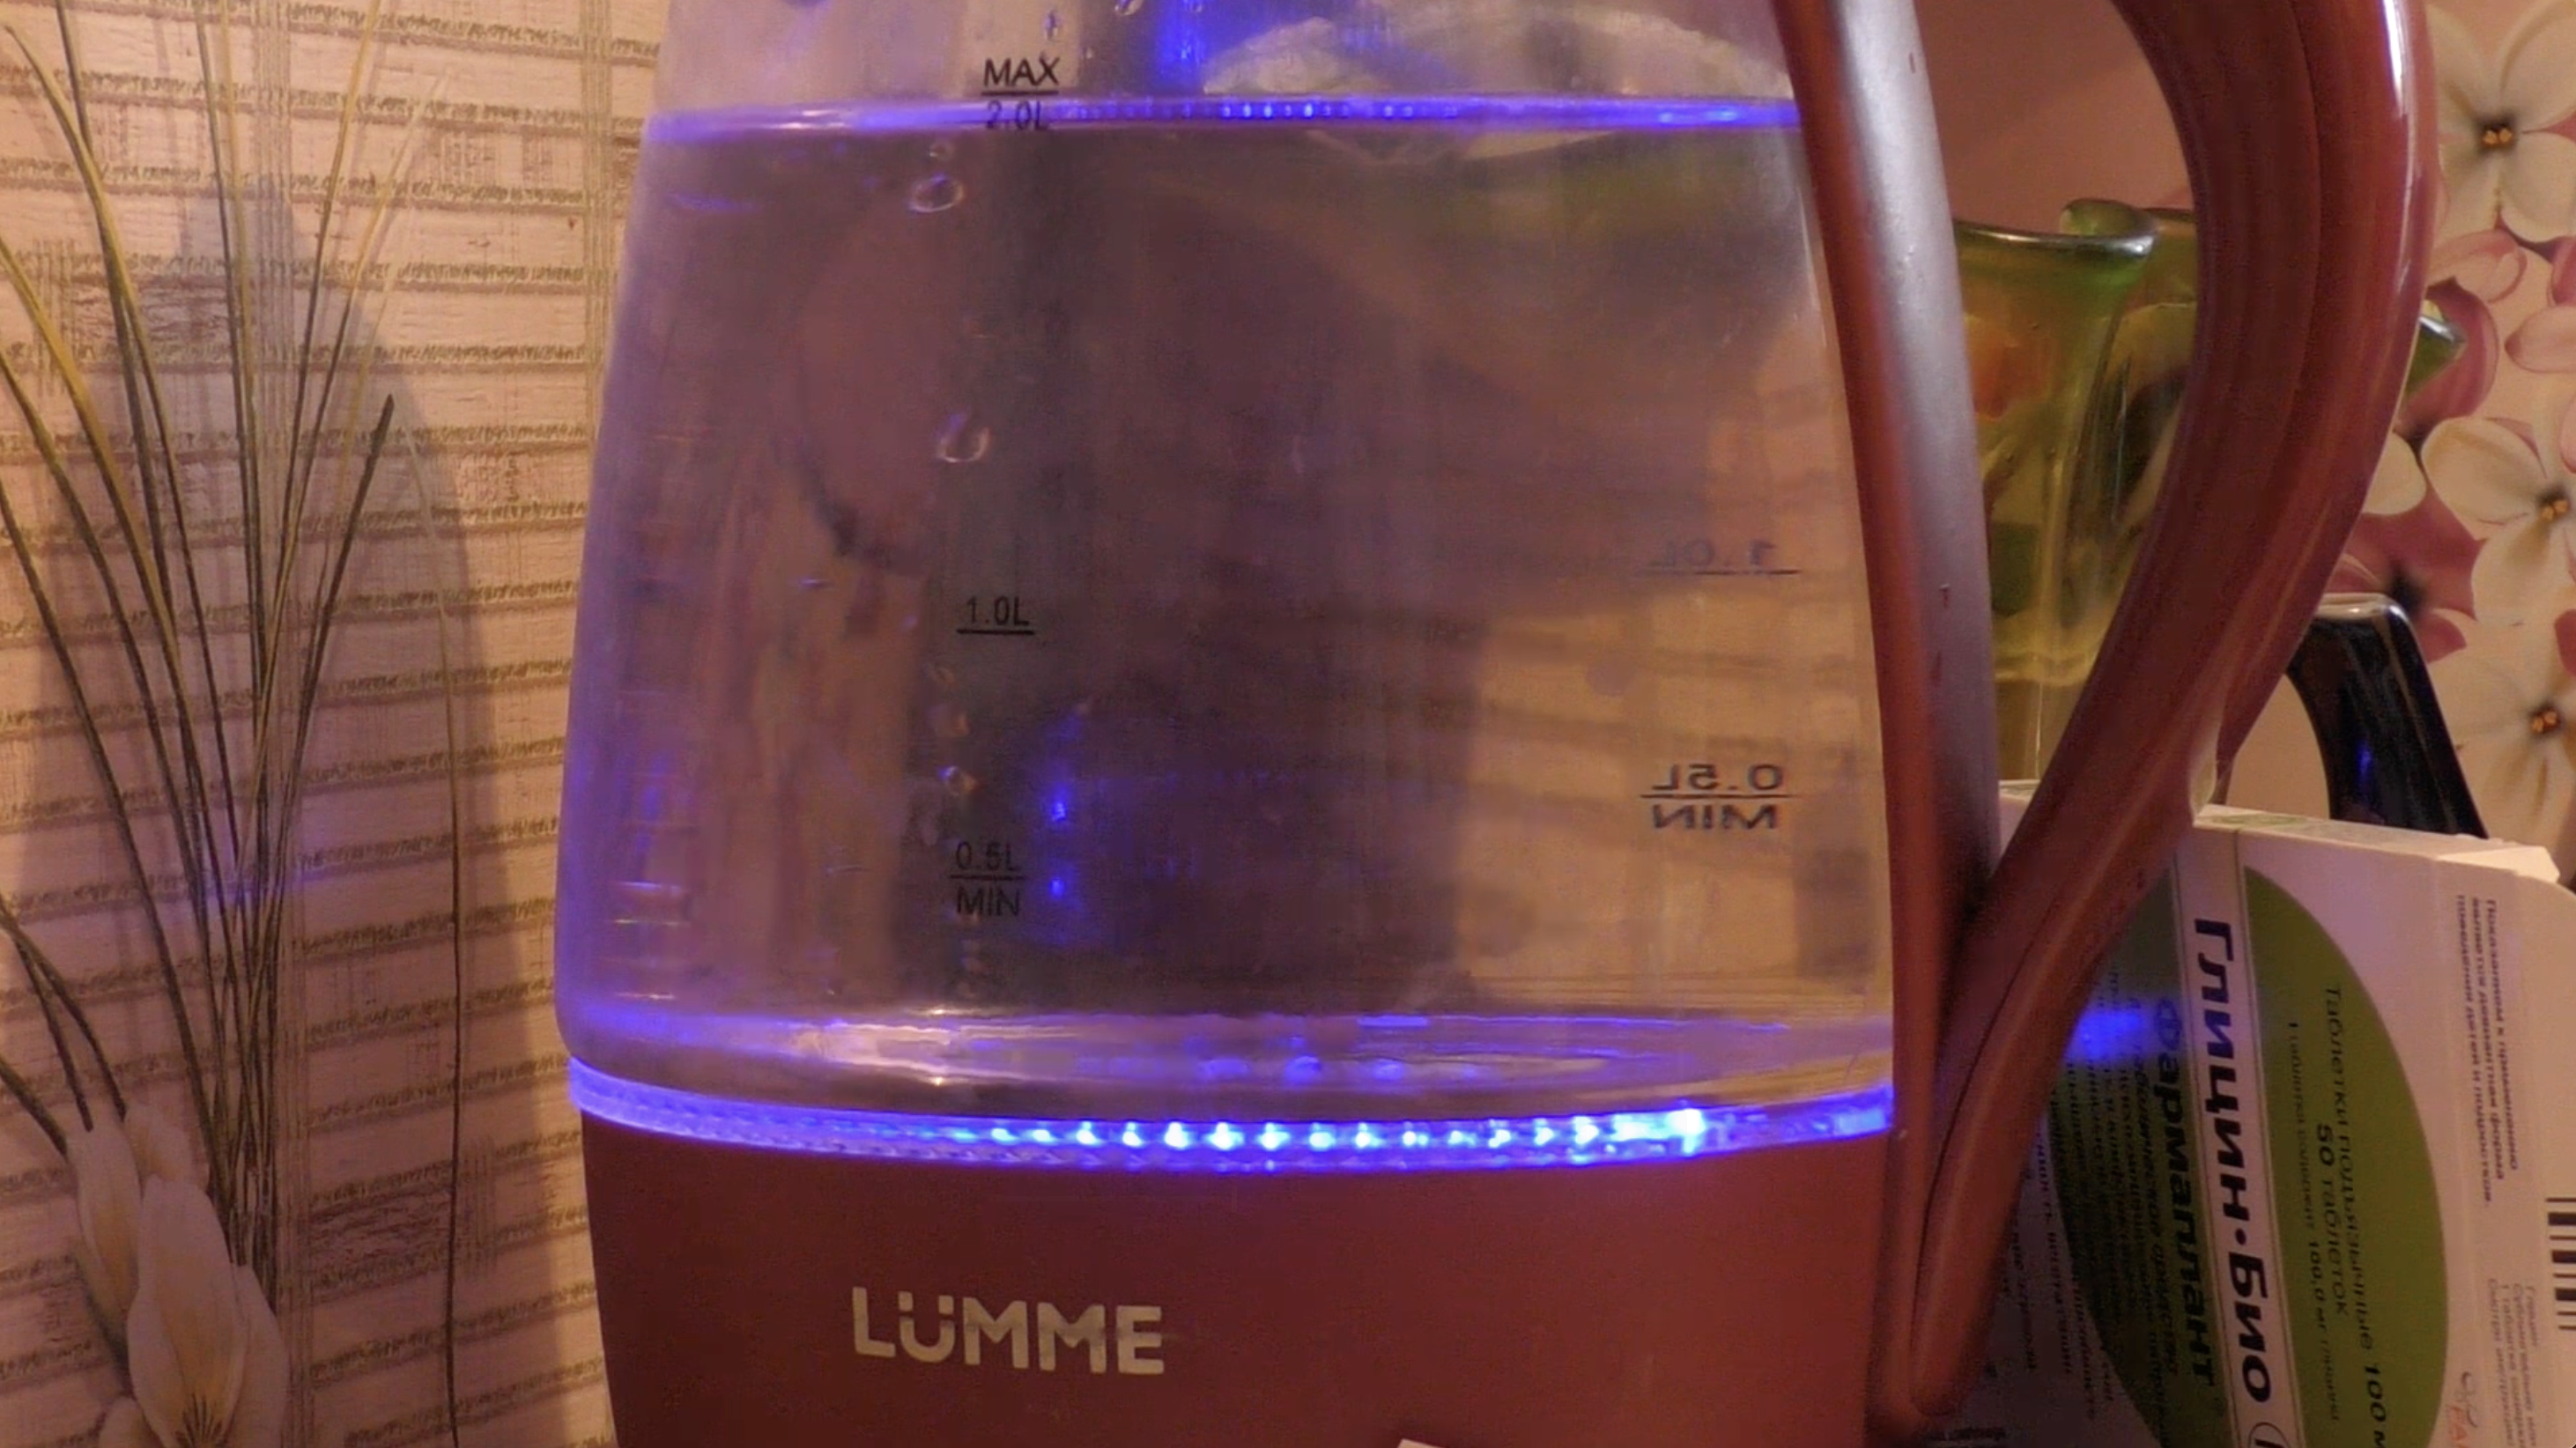
\includegraphics[width=0.8\textwidth]{img/image.png}
\caption{Лучший найденный маршрут в ЛР №6}
\end{figure}

\begin{figure}[H]
\centering
\includegraphics[width=0.8\textwidth]{img/image copy.png}
\caption{График сходимости решения}
\end{figure}

На Рис. 3 представлен график сходимости. Он показывает, как изменялась длина лучшего маршрута с каждой новой итерацией. Видно, что основные улучшения происходят в первые 25 итераций, после чего алгоритм постепенно уточняет решение и сходится к финальному результату.

\subsubsection{Выводы}
Муравьиный алгоритм успешно решил задачу коммивояжёра на наборе данных из 29 городов. Ключевые достижения:
\begin{itemize}
\item Получено решение с улучшением 0.07\% относительно генетического алгоритма из ЛР №3;
\item Показано незначительное улучшение по сравнению с генетическим алгоритмом;
\item Реализован эффективный критерий остановки по стагнации, что позволило завершить вычисления после 74 итераций;
\item Обеспечена стабильная сходимость алгоритма с последовательным улучшением качества решения;
\item Достигнуто время выполнения 2.15 секунд для задачи размерности 29 городов.
\end{itemize}
Алгоритм продемонстрировал хорошую производительность и способность находить близкие к оптимальным решения для задач средней размерности, подтвердив практическую применимость муравьиных алгоритмов для решения задач коммивояжёра.

\newpage
\section{Ответ на контрольный вопрос}
\textbf{Вопрос: }Как оценивается качество построенного решения в МА?

\textbf{Ответ: } Качество решения в муравьином алгоритме оценивается через \textbf{длину маршрута}:

\begin{equation}
L^k = \sum_{i=1}^{n-1} d(c_i, c_{i+1}) + d(c_n, c_1)
\end{equation}

где:
\begin{itemize}
\item $L^k$ -- длина маршрута муравья $k$
\item $d(c_i, c_j)$ -- расстояние между городами $i$ и $j$
\item $n$ -- количество городов
\end{itemize}

Чем меньше $L^k$, тем лучше решение. Лучшее решение на итерации:
\begin{equation}
L_{best} = \min(L^1, L^2, \dots, L^m)
\end{equation}
где $m$ -- количество муравьёв.

\newpage
\section*{Заключение}
\addcontentsline{toc}{section}{Заключение}
В результате выполнения лабораторной работы №3 были достигнуты следующие результаты:
\begin{itemize}
    \item освоен теоретический материал;
    \item создана программа на языке \texttt{Python} с использованием среды \texttt{Jupyter Notebook};
    \item реализован муравьиный алгоритм выводящий оптимальный маршут, а так же проведено сравнение с генетическим алгоритмом поиска оптимального пути.
    \item выводы алгоритма из работы №3 и работы №6, свидетельствуют о том, что, муравьиный алгоритм более эффективен, чем классический генетический алгоритм.  
\end{itemize}

\newpage
\section*{Список литературы}
\addcontentsline{toc}{section}{Список литературы}
\begin{enumerate}
  \item Методические указания по выполнению лабораторных работ к курсу <<Генетические алгоритмы>>, стр.~119.
\end{enumerate}

\newpage
\addcontentsline{toc}{section}{Приложение А}
\twosideheading{Исходный код}{Приложение А}
\begin{lstlisting}
    import numpy as np
import random
import math
import matplotlib.pyplot as plt

def load_cities_coords():
    coords_str = """1 20833.3333 17100.0000
2 20900.0000 17066.6667
3 21300.0000 13016.6667
4 21600.0000 14150.0000
5 21600.0000 14966.6667
6 21600.0000 16500.0000
7 22183.3333 13133.3333
8 22583.3333 14300.0000
9 22683.3333 12716.6667
10 23616.6667 15866.6667
11 23700.0000 15933.3333
12 23883.3333 14533.3333
13 24166.6667 13250.0000
14 25149.1667 12365.8333
15 26133.3333 14500.0000
16 26150.0000 10550.0000
17 26283.3333 12766.6667
18 26433.3333 13433.3333
19 26550.0000 13850.0000
20 26733.3333 11683.3333
21 27026.1111 13051.9444
22 27096.1111 13415.8333
23 27153.6111 13203.3333
24 27166.6667 9833.3333
25 27233.3333 10450.0000
26 27233.3333 11783.3333
27 27266.6667 10383.3333
28 27433.3333 12400.0000
29 27462.5000 12992.2222"""
    
    lines = coords_str.strip().split('\n')
    coords = []
    for line in lines:
        parts = line.strip().split()
        x, y = float(parts[1]), float(parts[2])
        coords.append((x, y))
    return np.array(coords)

def compute_distance_matrix(cities):
    n = len(cities)
    dist = np.zeros((n, n))
    for i in range(n):
        for j in range(i + 1, n):
            dx = cities[i][0] - cities[j][0]
            dy = cities[i][1] - cities[j][1]
            d = math.sqrt(dx * dx + dy * dy)
            dist[i][j] = d
            dist[j][i] = d
    return dist

class AntColonyTSP:
    def __init__(self, distances, n_ants=50, n_iterations=500, decay=0.3, alpha=1., beta=3., max_stagnation=30):
        self.distances = distances
        self.n_cities = len(distances)
        self.n_ants = n_ants
        self.n_iterations = n_iterations
        self.decay = decay
        self.alpha = alpha
        self.beta = beta
        self.max_stagnation = max_stagnation
        self.pheromone = np.ones((self.n_cities, self.n_cities)) * 0.1
        self.best_path = None
        self.best_length = float('inf')
        self.history = []
        self.stagnation_counter = 0

    def run(self):
        prev_best = float('inf')
        for it in range(self.n_iterations):
            all_paths = []
            for _ in range(self.n_ants):
                path = self._construct_solution()
                length = self._path_length(path)
                all_paths.append((path, length))
                if length < self.best_length:
                    self.best_length = length
                    self.best_path = path.copy()
            
            if self.best_length < prev_best:
                prev_best = self.best_length
                self.stagnation_counter = 0
            else:
                self.stagnation_counter += 1
            
            self._update_pheromone(all_paths)
            self.pheromone *= (1 - self.decay)
            self.history.append(self.best_length)
            
            print(f"Iteration {it + 1:3d}: Best length = {self.best_length:8.2f} (Stagnation: {self.stagnation_counter})")
            
            if self.stagnation_counter >= self.max_stagnation:
                print(f"\nAlgorithm stopped due to stagnation.")
                break
        
        return self.best_path, self.best_length, self.history

    def _construct_solution(self):
        start = random.randint(0, self.n_cities - 1)
        path = [start]
        visited = {start}
        current = start
        
        for _ in range(self.n_cities - 1):
            next_city = self._select_next(current, visited)
            if next_city is None:
                break
            path.append(next_city)
            visited.add(next_city)
            current = next_city
        
        path.append(start)
        return path

    def _select_next(self, current, visited):
        unvisited = [j for j in range(self.n_cities) if j not in visited]
        if not unvisited:
            return None
        
        pheromone = self.pheromone[current][unvisited]
        heuristic = np.array([1.0 / (self.distances[current][j] + 1e-10) for j in unvisited])
        probs = (pheromone ** self.alpha) * (heuristic ** self.beta)
        probs_sum = probs.sum()
        
        if probs_sum == 0:
            return random.choice(unvisited)
        
        probs /= probs_sum
        return np.random.choice(unvisited, p=probs)

    def _update_pheromone(self, all_paths):
        delta_pheromone = np.zeros_like(self.pheromone)
        for path, length in all_paths:
            for i in range(len(path) - 1):
                a, b = path[i], path[i + 1]
                delta_pheromone[a][b] += 1.0 / (length + 1e-10)
                delta_pheromone[b][a] += 1.0 / (length + 1e-10)
        self.pheromone += delta_pheromone

    def _path_length(self, path):
        total = 0.0
        for i in range(len(path) - 1):
            a, b = path[i], path[i + 1]
            total += self.distances[a][b]
        return total

def plot_tour_comparison(cities, found_tour, title="Tour"):
    plt.figure(figsize=(12, 8))
    
    x_found = [cities[i][0] for i in found_tour] + [cities[found_tour[0]][0]]
    y_found = [cities[i][1] for i in found_tour] + [cities[found_tour[0]][1]]
    plt.plot(x_found, y_found, 'o-', linewidth=1.2, markersize=5, color='blue', label='ACO')
    
    start_x, start_y = cities[found_tour[0]]
    plt.scatter(start_x, start_y, color='red', s=120, zorder=5, label='Start/Finish')
    
    for i, (x, y) in enumerate(cities):
        plt.text(x + 1, y + 1, str(i + 1), fontsize=6, ha='center', va='center', alpha=0.7)
    
    plt.title(title)
    plt.xlabel("X")
    plt.ylabel("Y")
    plt.legend()
    plt.grid(True, alpha=0.3)
    plt.tight_layout()
    plt.show()

def plot_convergence(history):
    plt.figure(figsize=(8, 5))
    plt.plot(history, 'b-', linewidth=1.5)
    plt.title("Convergence")
    plt.xlabel("Iteration")
    plt.ylabel("Best tour length")
    plt.grid(True, alpha=0.3)
    plt.tight_layout()
    plt.show()

if __name__ == "__main__":
    cities = load_cities_coords()
    dist_matrix = compute_distance_matrix(cities)
    
    aco = AntColonyTSP(dist_matrix, n_ants=50, n_iterations=500, decay=0.3, alpha=1.0, beta=3.0)
    best_path, best_length, history = aco.run()
    
    print(f"\nBest tour length: {best_length:.2f}")
    print(f"Best path: {[x+1 for x in best_path]}")
    
    plot_tour_comparison(cities, best_path, f"Best Tour (Length: {best_length:.2f})")
    plot_convergence(history)
\end{lstlisting}
\end{document}

